\documentclass[10pt,a4paper]{article}
\usepackage[T1]{fontenc}
\usepackage[utf8]{inputenc}
\usepackage{lmodern,amsmath,amssymb,microtype,xspace}
\usepackage[margin=22mm,headheight=14pt]{geometry}
\usepackage{graphicx,booktabs,tabularx,array,listings,caption,float,fancyhdr,titlesec}
\usepackage[dvipsnames]{xcolor}
\usepackage{tikz}
\usetikzlibrary{arrows.meta,positioning,fit,calc,matrix,decorations.pathreplacing}
\usepackage[colorlinks=true,linkcolor=MidnightBlue,urlcolor=MidnightBlue,citecolor=MidnightBlue]{hyperref}
\usepackage{bookmark}
\definecolor{Ink}{HTML}{17354B}
\definecolor{Scan}{HTML}{2A78D6}
\definecolor{Branch}{HTML}{EB6834}
\definecolor{Keys}{HTML}{1BAF7A}
\definecolor{Soft}{HTML}{F3F6F8}
\definecolor{Muted}{HTML}{898781}
\pagestyle{fancy}\fancyhf{}
\lhead{\small Searching Binary Embeddings}\rhead{\small\thepage}
\renewcommand{\headrulewidth}{0.3pt}
\setlength{\parindent}{0pt}\setlength{\parskip}{4pt}
\setlength{\emergencystretch}{2em}\raggedbottom
\titlespacing*{\section}{0pt}{12pt}{8pt}
\titlespacing*{\subsection}{0pt}{10pt}{5pt}
\titlespacing*{\subsubsection}{0pt}{8pt}{4pt}
\captionsetup{font=small,labelfont=bf,skip=5pt}
\lstset{basicstyle=\small\ttfamily,backgroundcolor=\color{Soft},frame=single,
 rulecolor=\color{gray!30},columns=fullflexible,keepspaces=true,
 showstringspaces=false,breaklines=true,aboveskip=6pt,belowskip=6pt}
\tikzset{box/.style={draw=Ink!50,fill=Soft,rounded corners=2pt,align=center,
 minimum height=9mm,font=\small,text=Ink},arr/.style={-{Latex[length=2mm]},draw=Ink!60},
 scan/.style={box,draw=Scan,fill=Scan!10},branch/.style={box,draw=Branch,fill=Branch!10},
 keys/.style={box,draw=Keys,fill=Keys!12},
 cell/.style={draw=Ink!40,minimum width=5.5mm,minimum height=5.5mm,inner sep=0pt,font=\footnotesize,anchor=center},
 hot/.style={cell,fill=Branch!25},cold/.style={cell,fill=Soft}}
\newcommand{\ceil}[1]{\left\lceil #1\right\rceil}
\newcommand{\E}{\mathbb E}
\newcolumntype{Y}{>{\raggedright\arraybackslash}X}
\hypersetup{pdftitle={Searching Binary Embeddings: Three Methods on One Dataset},
 pdfsubject={Scan, bitplanes and backward walk compared on the same documents and queries}}
\begin{document}
{\Large\bfseries\color{Ink} Searching Binary Embeddings}\par
{\large Three methods, one dataset}\par
{\small 12 September 2026}\par
\begin{abstract}
Exa stores document embeddings as short binary codes, groups them into clusters, and scores
the documents of a few clusters with a lookup table. This report asks whether two extra
index structures can reduce that scoring work: \emph{Bitplanes}, which split a cluster by
one sign bit at a time, and \emph{Backward Walk}, which looks up documents by a short key.
We derive the time, memory and recall of all three methods, use the formulas to choose each
method's best settings, and then measure every setting on one fixed dataset: one million
MS~MARCO passages and 200 queries. Only the index parameters change between runs. The
formulas predict the recorded operation counts exactly and the measured search times within
a few percent. On this dataset the original method is fastest at every recall target, and
the calculations show why: on real embeddings, one sign bit removes only about 15\% of the
documents, while a cluster boundary removes about 98\%. The same formulas also state the
conditions under which Bitplanes or Backward Walk would win.
\end{abstract}

\section{Introduction}
\subsection{Exa's method, end to end}
We build on the search pipeline that Exa describes in its engineering blog~\cite{exa}. That
post explains each technique in detail, so we only name the steps here and refer the reader
to it. A document is embedded, the embedding is shortened by keeping its first values, which Matryoshka training makes possible~\cite{mrl}, and each
of the remaining $d$ values is replaced by one bit: 1 if the value is positive, 0 if it is
negative. This is Exa's \emph{binary quantization}. The binary codes are grouped into $C$
clusters. When a query arrives, the system keeps the query in floating point, selects the $P$
clusters whose centres are closest, and scores every document in those clusters with a lookup
table that handles four bits at a time. The best documents can then be reranked with full
vectors. Figure~\ref{fig:pipeline} shows the sequence; the blue box is the step that this
report studies.

\begin{figure}[H]\centering
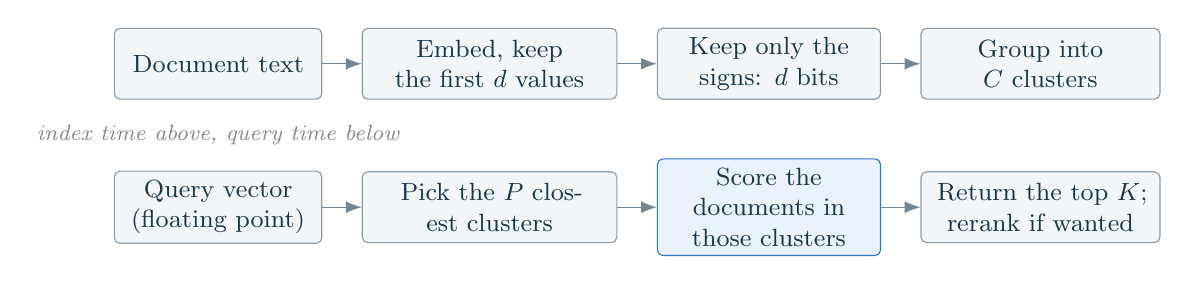
\begin{tikzpicture}[node distance=5mm and 5mm]
\node[box,text width=24mm] (text) {Document text};
\node[box,text width=30mm,right=of text] (embed) {Embed, keep the first $d$ values};
\node[box,text width=26mm,right=of embed] (bits) {Keep only the signs: $d$ bits};
\node[box,text width=28mm,right=of bits] (store) {Group into $C$ clusters};
\draw[arr] (text)--(embed);\draw[arr] (embed)--(bits);\draw[arr] (bits)--(store);
\node[box,text width=24mm,below=9mm of text] (q) {Query vector\\(floating point)};
\node[box,text width=30mm,right=of q] (route) {Pick the $P$ closest clusters};
\node[scan,text width=26mm,right=of route] (local) {Score the documents in those clusters};
\node[box,text width=28mm,right=of local] (out) {Return the top $K$;\\rerank if wanted};
\draw[arr] (q)--(route);\draw[arr] (route)--(local);\draw[arr] (local)--(out);
\node[font=\footnotesize\itshape,text=Muted] at ($(text.south)!0.5!(q.north)$) {index time above, query time below};
\end{tikzpicture}
\caption{Exa's pipeline as described in~\cite{exa}. The top row happens once, when documents
are indexed. The bottom row happens for every query. The blue box, scoring the documents of
the opened clusters, is the step that the two new methods try to shorten. We call the
unchanged pipeline \textbf{method A}, the original method.}
\label{fig:pipeline}
\end{figure}

Two numbers describe the scoring step. With $N$ documents in $C$ clusters of roughly equal
size, opening $P$ clusters means scoring about $NP/C$ documents. For one million documents,
4096 clusters and one opened cluster, that is about 244 documents. Opening more clusters finds
more of the true answers but scores more documents. The rest of this report is about that
trade.

\subsection{Idea background}
The query tells us exactly which document code would score best. Take a small query with
five values,
\[
 q=[\,0.7,\ 0.5,\ -0.4,\ -0.6,\ 0.3\,].
\]
A document bit of 1 stands for $+1$ and a bit of 0 stands for $-1$; the score is the sum of
$q_i$ times the document's $\pm1$ at each position. At the first position the query value is
$0.7$, so a document bit of 1 contributes $+0.7$ and a bit of 0 contributes $-0.7$. At the
third position the query value is $-0.4$, so now a bit of 0 is better. Following this rule at
every position gives the pattern \texttt{11001}, and its score is
$0.7+0.5+0.4+0.6+0.3=2.5$. No document can score higher.

Every other code loses some of that score. A document whose bit disagrees with the query
sign at position $i$ loses $2|q_i|$: instead of gaining $|q_i|$ it pays $|q_i|$. If we call
the sum of the query weights at the disagreeing positions the \emph{penalty} $p$, then
\begin{equation}
 S(q,b)=Q-2p,\qquad Q=\sum_i|q_i|,\qquad p=\sum_{i:\ b_i\ne\operatorname{sign}(q_i)}|q_i|.
 \label{eq:score}
\end{equation}
The code \texttt{11000} disagrees only at the last position, so its penalty is $0.3$ and its
score is $2.5-0.6=1.9$. The code \texttt{01001} disagrees only at the first position, which
carries the largest weight; its score is $2.5-1.4=1.1$. Position matters: a mismatch on a
large query value costs more than a mismatch on a small one.

This suggests a question. Method A scores every document in the opened clusters, even the
ones that disagree with the query on its largest weights. \emph{What if the index let us go
straight to the documents whose codes are close to the preferred pattern, and skip the
rest?} Two structures do this in different ways. Bitplanes split the documents by one sign
bit at a time, largest query weight first. Backward Walk stores documents under a short key
and visits the keys in order of increasing penalty. Both keep Exa's scoring rule and its
clusters; they change only the blue box of Figure~\ref{fig:pipeline}.

We use the six documents in Table~\ref{tab:toy} as a running example, together with the
query above and $K=2$ results wanted. Scoring all six documents is what method A does. The
best two are documents 0 and 1, with scores 2.5 and 1.9.

\begin{table}[H]\centering\small
\caption{Six example documents with five sign bits each, scored against
$q=[0.7,0.5,-0.4,-0.6,0.3]$. The penalty adds the query weights at the positions where the
document disagrees with the query sign.}
\label{tab:toy}
\begin{tabular}{@{}clcc@{}}\toprule
ID & Code & Disagreeing positions (weights) & Score $=2.5-2p$\\\midrule
0 & \texttt{11001} & none & 2.5\\
1 & \texttt{11000} & 5 (0.3) & 1.9\\
2 & \texttt{10100} & 2, 3, 5 (0.5, 0.4, 0.3) & 0.1\\
3 & \texttt{01001} & 1 (0.7) & 1.1\\
4 & \texttt{11101} & 3 (0.4) & 1.7\\
5 & \texttt{00110} & all five (2.5) & $-2.5$\\\bottomrule
\end{tabular}
\end{table}

\subsection{Two new methods: Bitplanes and Backward Walk}
\subsubsection{Bitplanes}
Method A stores each document as one row of bits. Bitplanes, which we call \textbf{method B},
additionally store the same bits sideways: one row per bit position, one column per document,
inside each cluster. Figure~\ref{fig:bitplane-index} shows both layouts for the example. The
sideways row for position 1 is \texttt{111010}; it says that documents 0, 1, 2 and 4 have a 1
there. Such a row is called a \emph{bitplane}. With 64-bit words, one bitplane for a cluster
of $n$ documents occupies $\lceil n/64\rceil$ words, and the cluster needs $d$ of them.

\begin{figure}[H]\centering
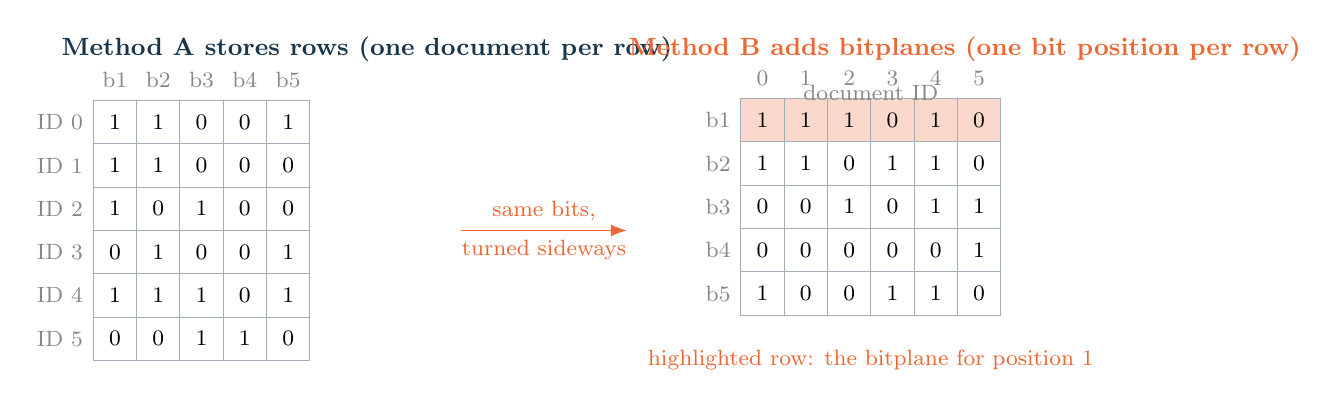
\begin{tikzpicture}
\node[anchor=west,font=\small\bfseries,text=Ink] at (0,3.2) {Method A stores rows (one document per row)};
\matrix (rows) at (1.9,0.9) [matrix of nodes,nodes={cell},column sep=-\pgflinewidth,row sep=-\pgflinewidth]{
 1&1&0&0&1\\ 1&1&0&0&0\\ 1&0&1&0&0\\ 0&1&0&0&1\\ 1&1&1&0&1\\ 0&0&1&1&0\\};
\foreach \i/\l in {1/0,2/1,3/2,4/3,5/4,6/5}{\node[font=\footnotesize,text=Muted,anchor=east] at (rows-\i-1.west) {ID \l\ };}
\node[font=\footnotesize,text=Muted] at (rows-1-1.north) [above=1pt] {b1};
\node[font=\footnotesize,text=Muted] at (rows-1-2.north) [above=1pt] {b2};
\node[font=\footnotesize,text=Muted] at (rows-1-3.north) [above=1pt] {b3};
\node[font=\footnotesize,text=Muted] at (rows-1-4.north) [above=1pt] {b4};
\node[font=\footnotesize,text=Muted] at (rows-1-5.north) [above=1pt] {b5};
\node[anchor=west,font=\small\bfseries,text=Branch] at (7.2,3.2) {Method B adds bitplanes (one bit position per row)};
\matrix (planes) at (10.4,1.2) [matrix of nodes,nodes={cell},column sep=-\pgflinewidth,row sep=-\pgflinewidth]{
 |[hot]|1&|[hot]|1&|[hot]|1&|[hot]|0&|[hot]|1&|[hot]|0\\ 1&1&0&1&1&0\\ 0&0&1&0&1&1\\ 0&0&0&0&0&1\\ 1&0&0&1&1&0\\};
\foreach \i/\l in {1/b1,2/b2,3/b3,4/b4,5/b5}{\node[font=\footnotesize,text=Muted,anchor=east] at (planes-\i-1.west) {\l\ };}
\foreach \j/\l in {1/0,2/1,3/2,4/3,5/4,6/5}{\node[font=\footnotesize,text=Muted] at (planes-1-\j.north) [above=1pt] {\l};}
\node[font=\footnotesize,text=Muted] at (10.4,2.65) {document ID};
\node[font=\footnotesize,text=Branch] at (10.4,-0.75) {highlighted row: the bitplane for position 1};
\draw[arr,Branch] (5.2,0.9) -- node[above,font=\footnotesize,text=Branch]{same bits,} node[below,font=\footnotesize,text=Branch]{turned sideways} (7.3,0.9);
\end{tikzpicture}
\caption{The two layouts of the same six codes. Method A keeps only the rows on the left.
Method B keeps the rows for scoring and adds the bitplanes on the right for splitting. The
highlighted bitplane belongs to position 1, which has the largest query weight.}
\label{fig:bitplane-index}
\end{figure}

Searching uses the bitplanes to narrow down the candidates before scoring
(Figure~\ref{fig:bitplane-search}). We start with a \emph{mask} that marks every document
in the cluster as a candidate: \texttt{111111}. We take the position with the largest query
weight, position 1 with $0.7$, where the query prefers a 1. One AND between the mask and the
bitplane for position 1 gives the documents that agree, \texttt{111010}, which are documents
0, 1, 2 and 4. The remaining documents, 3 and 5, disagree at a position of weight $0.7$, so
every document in that group carries a penalty of at least $0.7$. We keep that group aside
in a queue, labelled with its penalty, and continue with the agreeing group.

The next largest weight is position 4 ($0.6$, prefers 0). All four remaining documents have
a 0 there, so nothing is removed. Position 2 ($0.5$, prefers 1) separates document 2 from
documents 0, 1 and 4. When a group is small enough, which we call the \emph{leaf size}, we
stop splitting and score its documents with the same lookup table as method A. Scoring
documents 0, 1 and 4 gives $2.5$, $1.9$ and $1.7$; the best two are 2.5 and 1.9.

Now the queue decides whether any stored group needs attention. Equation~\ref{eq:score} gives
each group a ceiling: a group with penalty $p$ cannot contain a score above $Q-2p$. The group
$\{2\}$ has penalty $0.5$ and ceiling $1.5$, and the group $\{3,5\}$ has penalty $0.7$ and
ceiling $1.1$. Both ceilings are below $1.9$, the worse of the two scores we already hold, so
neither group can change the answer. The search ends having scored three documents instead
of six, with exactly the answer that method A returns.

\begin{figure}[H]\centering
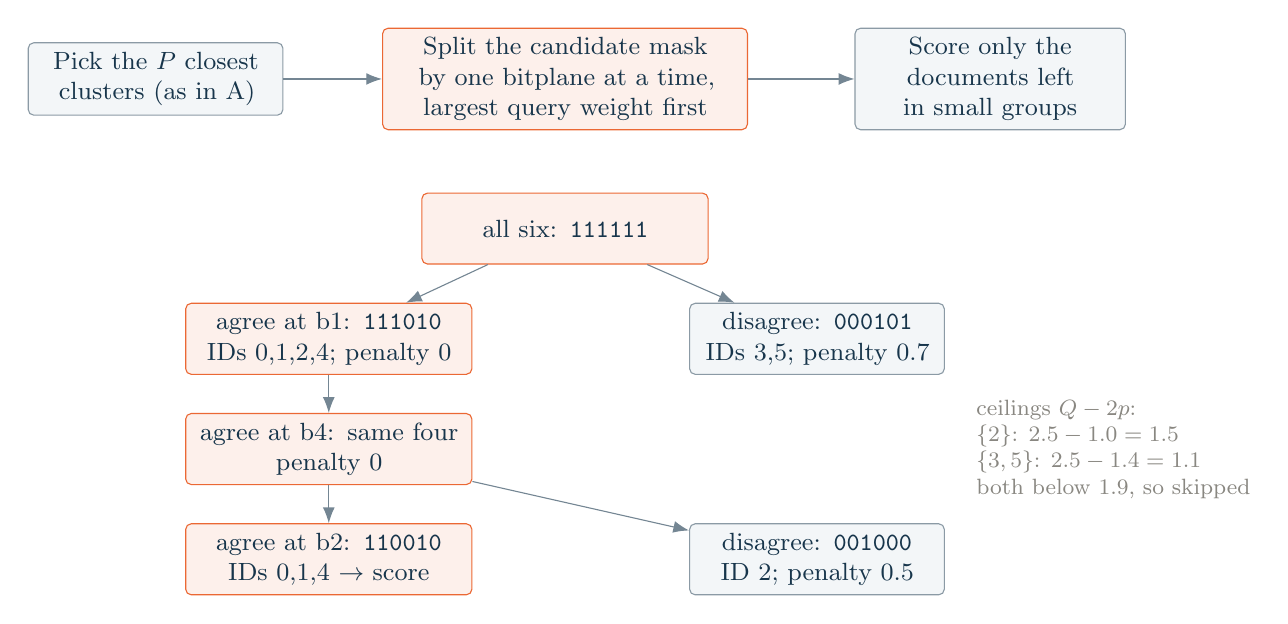
\begin{tikzpicture}[node distance=4mm]
\node[box,text width=30mm] (route) at (0,0) {Pick the $P$ closest clusters (as in A)};
\node[branch,text width=44mm] (split) at (5.2,0) {Split the candidate mask by one bitplane at a time, largest query weight first};
\node[box,text width=32mm] (score) at (10.6,0) {Score only the documents left in small groups};
\draw[arr] (route)--(split);\draw[arr] (split)--(score);
\node[branch,text width=34mm] (m0) at (5.2,-1.9) {all six: \texttt{111111}};
\node[branch,text width=34mm] (m1) at (2.2,-3.3) {agree at b1: \texttt{111010}\\IDs 0,1,2,4; penalty 0};
\node[box,text width=30mm] (m1x) at (8.4,-3.3) {disagree: \texttt{000101}\\IDs 3,5; penalty 0.7};
\node[branch,text width=34mm] (m2) at (2.2,-4.7) {agree at b4: same four\\penalty 0};
\node[branch,text width=34mm] (m3) at (2.2,-6.1) {agree at b2: \texttt{110010}\\IDs 0,1,4 $\rightarrow$ score};
\node[box,text width=30mm] (m3x) at (8.4,-6.1) {disagree: \texttt{001000}\\ID 2; penalty 0.5};
\draw[arr] (m0)--(m1);\draw[arr] (m0)--(m1x);\draw[arr] (m1)--(m2);\draw[arr] (m2)--(m3);\draw[arr] (m2)--(m3x);
\node[font=\footnotesize,text=Muted,align=left,anchor=west] at (10.3,-4.7) {ceilings $Q-2p$:\\$\{2\}$: $2.5-1.0=1.5$\\$\{3,5\}$: $2.5-1.4=1.1$\\both below 1.9, so skipped};
\end{tikzpicture}
\caption{Method B on the example. Orange marks the changed step and the groups that the
search follows. Each split keeps the disagreeing group in a queue with its penalty. After
scoring the small group, the queued groups are dropped because their ceilings are below the
second-best score already found.}
\label{fig:bitplane-search}
\end{figure}

\begin{lstlisting}
bitplanes(query, opened_clusters, K, leaf_size, node_budget):
    table = score_table(query); best = top_k(K)
    order = positions sorted by |query value|, largest first
    queue = one full mask per opened cluster, penalty 0
    while queue is not empty:
        group = pop the group with the smallest penalty
        if Q - 2*group.penalty < best.worst_score(): break  # no group can win
        if visited groups == node_budget: break              # optional limit
        if group.count <= leaf_size or no positions remain:
            score every document in group.mask with table; offer to best
        else:
            agree, disagree = split group.mask by the bitplane of the next position
            push agree (same penalty); push disagree (penalty + |query value|)
    return best
\end{lstlisting}

Two settings control method B. The \emph{leaf size} decides when a group is small enough to
score. The \emph{node budget} caps how many groups the search may visit; with no budget, the
ceiling rule alone stops the search, and the answer is then the same as method A's within the
opened clusters. Both children of a split are as wide as the whole cluster: a mask of
$\lceil n/64\rceil$ words stays that wide even when only a few bits remain set. This is the
main cost of method B, and Section~2 counts it.

\subsubsection{Backward Walk}
The second structure, which we call \textbf{method C}, makes the ``go straight to the
preferred pattern'' idea literal. Choose $h$ fixed bit positions and read a document's bits
at those positions as a short \emph{key}. Inside each cluster, sort the documents by key so
that documents with the same key sit next to each other, and keep a small \emph{directory}
that maps each key to the start and length of its row range. Figure~\ref{fig:key-index}
shows this for the example with positions 2 and 3 as the key.

\begin{figure}[H]\centering
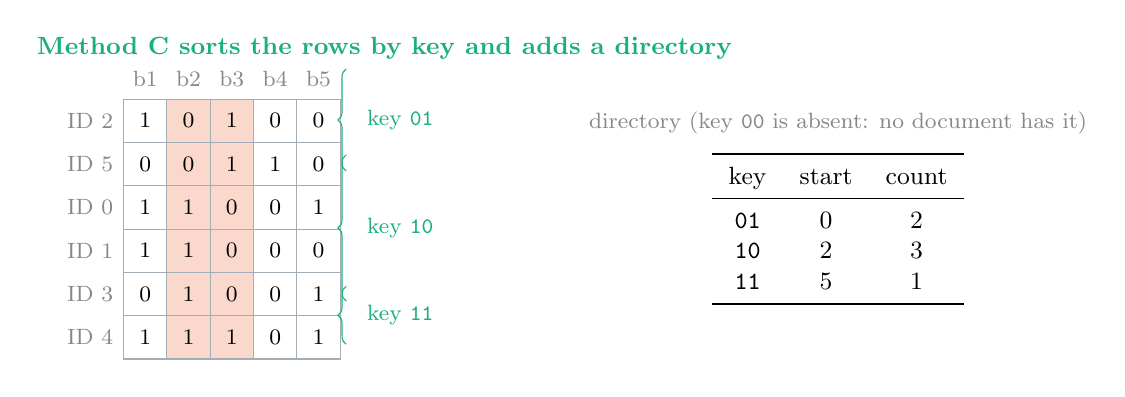
\begin{tikzpicture}
\node[anchor=west,font=\small\bfseries,text=Keys] at (0,3.3) {Method C sorts the rows by key and adds a directory};
\matrix (rows) at (2.6,1.0) [matrix of nodes,nodes={cell},column sep=-\pgflinewidth,row sep=-\pgflinewidth]{
 1&|[hot]|0&|[hot]|1&0&0\\ 0&|[hot]|0&|[hot]|1&1&0\\ 1&|[hot]|1&|[hot]|0&0&1\\ 1&|[hot]|1&|[hot]|0&0&0\\ 0&|[hot]|1&|[hot]|0&0&1\\ 1&|[hot]|1&|[hot]|1&0&1\\};
\foreach \i/\l in {1/2,2/5,3/0,4/1,5/3,6/4}{\node[font=\footnotesize,text=Muted,anchor=east] at (rows-\i-1.west) {ID \l\ };}
\foreach \j/\l in {1/b1,2/b2,3/b3,4/b4,5/b5}{\node[font=\footnotesize,text=Muted] at (rows-1-\j.north) [above=1pt] {\l};}
\draw[decorate,decoration={brace,amplitude=3pt},Keys] (rows-2-5.east) ++(2pt,-2.5pt) -- ++(0,5.6mm+5.6mm+5pt) node[midway,right=4pt,font=\footnotesize,text=Keys] {key \texttt{01}};
\draw[decorate,decoration={brace,amplitude=3pt},Keys] (rows-5-5.east) ++(2pt,-2.5pt) -- ++(0,3*5.6mm+5pt) node[midway,right=4pt,font=\footnotesize,text=Keys] {key \texttt{10}};
\draw[decorate,decoration={brace,amplitude=3pt},Keys] (rows-6-5.east) ++(2pt,-2.5pt) -- ++(0,5.6mm+5pt) node[midway,right=4pt,font=\footnotesize,text=Keys] {key \texttt{11}};
\node[align=center,font=\small] at (10.3,1.0) {\begin{tabular}{ccc}\toprule
key & start & count\\\midrule
\texttt{01} & 0 & 2\\
\texttt{10} & 2 & 3\\
\texttt{11} & 5 & 1\\\bottomrule
\end{tabular}};
\node[font=\footnotesize,text=Muted] at (10.3,2.35) {directory (key \texttt{00} is absent: no document has it)};
\end{tikzpicture}
\caption{The index of method C for the example, with bit positions 2 and 3 as the key
(highlighted). Rows are stored in key order, so the documents of one key form one contiguous
range. The directory holds one entry per key that occurs. The row IDs double as the list of
documents, so no separate posting list is needed.}
\label{fig:key-index}
\end{figure}

At query time we form the query's preferred key from the same positions. The query prefers
a 1 at position 2 and a 0 at position 3, so its key is \texttt{10}. A directory lookup returns
documents 0, 1 and 3, and we score them: $2.5$, $1.9$ and $1.1$. If this were enough we would
stop; but the best documents may have a different key, so the search must be able to move on.
It does so by walking away from the preferred key one flipped position at a time, cheapest
flip first, which is why we call it a backward walk (Figure~\ref{fig:key-walk}). Flipping
position 3 (weight $0.4$) gives key \texttt{11} with penalty $0.4$; flipping position 2
(weight $0.5$) gives \texttt{00} with penalty $0.5$; flipping both gives \texttt{01} with
penalty $0.9$. As in method B, a key with penalty $p$ has ceiling $Q-2p$. The next key,
\texttt{11}, has ceiling $2.5-0.8=1.7$, which is below the second-best score $1.9$ that we
already hold. The walk stops after scoring three documents, again with method A's answer.

\begin{figure}[H]\centering
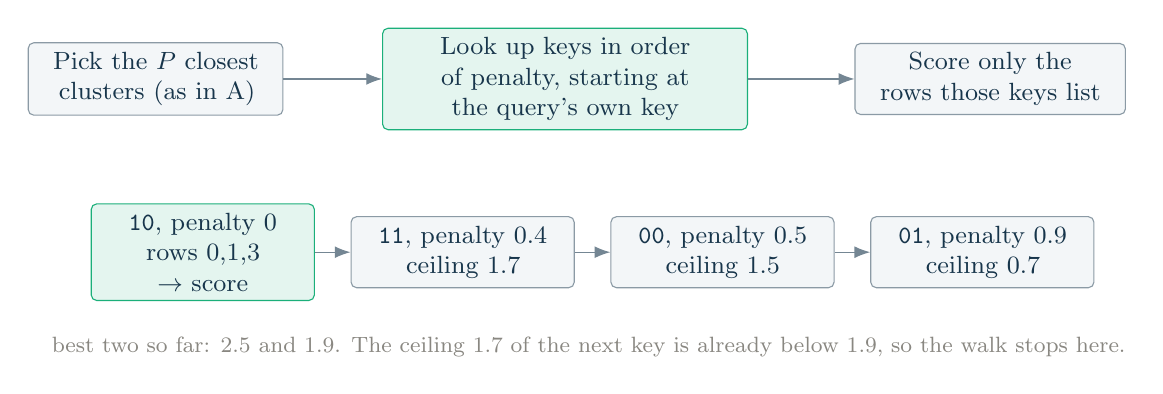
\begin{tikzpicture}[node distance=4mm]
\node[box,text width=30mm] (route) at (0,0) {Pick the $P$ closest clusters (as in A)};
\node[keys,text width=44mm] (walk) at (5.2,0) {Look up keys in order of penalty, starting at the query's own key};
\node[box,text width=32mm] (score) at (10.6,0) {Score only the rows those keys list};
\draw[arr] (route)--(walk);\draw[arr] (walk)--(score);
\node[keys,text width=26mm] (k0) at (0.6,-2.2) {\texttt{10}, penalty 0\\rows 0,1,3 $\rightarrow$ score};
\node[box,text width=26mm] (k1) at (3.9,-2.2) {\texttt{11}, penalty 0.4\\ceiling 1.7};
\node[box,text width=26mm] (k2) at (7.2,-2.2) {\texttt{00}, penalty 0.5\\ceiling 1.5};
\node[box,text width=26mm] (k3) at (10.5,-2.2) {\texttt{01}, penalty 0.9\\ceiling 0.7};
\draw[arr] (k0)--(k1);\draw[arr] (k1)--(k2);\draw[arr] (k2)--(k3);
\node[font=\footnotesize,text=Muted,align=center] at (5.5,-3.4) {best two so far: 2.5 and 1.9. The ceiling 1.7 of the next key is already below 1.9, so the walk stops here.};
\end{tikzpicture}
\caption{Method C on the example. Green marks the changed step. Keys are visited in
increasing penalty; each visit is one directory lookup per opened cluster. The walk stops as
soon as the next key's ceiling cannot beat the $K$th best score.}
\label{fig:key-walk}
\end{figure}

\begin{lstlisting}
backward_walk(query, opened_clusters, K, key_positions):
    table = score_table(query); best = top_k(K)
    keys = every key, ordered by penalty against the query's preferred key
    for key, penalty in keys:
        if Q - 2*penalty < best.worst_score(): break  # no key can win
        for cluster in opened_clusters:
            rows = cluster.directory.lookup(key)        # may be empty
            score each row with table; offer to best
    return best
\end{lstlisting}

Method C has one main setting, the key width $h$. There are $2^h$ possible keys. A wide key
makes each key's row range small but multiplies the number of keys the walk may have to
visit; a narrow key does the opposite. The key positions are fixed when the index is built,
so they cannot follow each query's largest weights the way method B's split order does. The
positions the enumeration visits are ordered by the query weights at those $h$ positions only.

Both new methods return exactly method A's answer within the opened clusters when they run to
completion, because the ceiling rule never drops a group or key that could still hold a
top-$K$ document. They can be faster only if the ceilings let them skip enough documents to
pay for the extra reads. Section~2 counts that work, Section~3 uses the counts to choose each
method's settings on the dataset, and Section~4 measures the result.

\section{Preliminary calculations}
This section counts what each method does for one query. The counts use the quantities in
Table~\ref{tab:symbols}. Section~4 records the same counts from the running code, so every
formula here is checked against the implementation.

\begin{table}[H]\centering\small
\caption{Quantities used in the calculations, with the values of the experiment where fixed.}
\label{tab:symbols}
\begin{tabularx}{\linewidth}{@{}lYl@{}}\toprule
Symbol & Meaning & In the experiment\\\midrule
$N$ & documents in the collection & 1,000,000\\
$d$ & bits per document code & 256\\
$K$ & results returned per query & 100\\
$C$, $P$ & clusters in the index; clusters opened for a query & chosen per method\\
$n_c$ & documents in cluster $c$ & from the data\\
$W_c=\lceil n_c/64\rceil$ & 64-bit words in one mask or bitplane of cluster $c$ & from the data\\
$L$ & leaf size of method B: a group this small is scored & chosen\\
$h$ & key width of method C, in bits & chosen\\
$Q=\sum_i|q_i|$ & total query weight; the best possible score & per query\\
$g$ & gap: the penalty of the $K$th best document, $(Q-S_K)/2$ & per query\\
$c_{\cdot}$ & milliseconds per counted operation (measured in Section~4) & measured\\\bottomrule
\end{tabularx}
\end{table}

\subsection{Time complexity}
Every method first selects $P$ clusters, which costs $T_{\rm route}$ and is the same for all
three at the same $C$ and $P$. We therefore concentrate on what happens inside the opened
clusters.

\subsubsection{Original method}
Method A scores every document in the opened clusters. Writing $F_A$ for that number,
\[
 F_A=\sum_{c\ \text{opened}}n_c\approx\frac{NP}{C},\qquad
 T_A=T_{\rm route}+c_{\rm call}+c_{\rm score}F_A.
\]
One score reads $d/4=64$ table entries and offers the result to a heap that keeps the best
$K$. The constant $c_{\rm score}$ covers both. $c_{\rm call}$ is the fixed cost of one call:
building the $64\times16$ lookup table and returning the sorted result. For one million
documents in 4096 clusters, opening one cluster scores about 244 documents; opening 1330
clusters, which Section~3 shows is needed for 99\% recall, scores about 322,000.

\subsubsection{Bitplanes}
Method B replaces some scoring by mask work. A split of a group in cluster $c$ reads
$W_c$ words of one bitplane and writes two child masks of $W_c$ words each. If the search
performs $J_c$ splits in cluster $c$ and scores $E_c$ groups there, it visits
\[
 V_s=\sum_c J_cW_c\ \text{split words},\qquad
 V_l=\sum_c E_cW_c\ \text{leaf words}.
\]
The leaf words are read to find which bits are still set before scoring those documents.
Both counts use the full width $W_c$: a group that has shrunk to 80 documents inside a
cluster of 6,400 still has a mask of $100$ words, and the next split reads all 100.
With $F_B$ documents scored and $G$ groups taken from the queue,
\[
 T_B=T_{\rm route}+c_{\rm call}+c_{\rm score}F_B+c_{\rm split}V_s+c_{\rm leaf}V_l+c_{\rm group}G.
\]
$c_{\rm group}$ prices the queue operations and the allocation of the two child masks. When
$L\ge n_c$ for every opened cluster, no split happens: $V_s=0$, $V_l=\sum_c W_c$,
$G=P$, and $F_B=F_A$. Method B then does method A's work plus one pass over the masks.

\subsubsection{Backward Walk}
Method C replaces scoring by directory lookups. Each key it visits costs one lookup in each
opened cluster, and an absent key still costs the lookup. With $E$ keys visited,
\[
 H=EP\ \text{lookups},\qquad
 T_C=T_{\rm route}+c_{\rm call}+c_{\rm score}F_C+c_{\rm lookup}H+c_{\rm key}E.
\]
$c_{\rm key}$ prices generating the next key in penalty order. If the ceiling rule never
stops the walk, it visits every key: $E=2^h$ and $F_C=F_A$. With $h=8$ and 1330 opened
clusters that is $256\times1330\approx340{,}000$ lookups on top of method A's scoring.

\subsection{Memory complexity}
We separate the index, which is held permanently, from the working memory of one query.

\subsubsection{Original method}
Each code occupies $d/8=32$ bytes and each document ID 8 bytes:
\[
 M_A=N(32+8)\ \text{bytes}=40\ \text{MB at }N=10^6,
\]
plus the cluster centres, $4Cd$ bytes ($4$~MB for $C=4096$). A query needs the lookup
table ($64\times16$ doubles, 8~KB) and the heap of $K$ results.

\subsubsection{Bitplanes}
Method B keeps method A's rows and adds $d$ bitplanes per cluster:
\[
 M_B=M_A+8d\sum_{c=1}^{C}W_c\ \text{bytes}.
\]
For one cluster of one million documents, $\sum_c W_c=15{,}625$ and the planes add
$8\times256\times15{,}625=32$~MB, making 72~MB. With 4096 clusters of about 238 documents
each mask is padded to whole words, so $\sum_c W_c$ rises to about 16,400 and the planes to
about 33.6~MB. During a query, every group waiting in the queue holds a mask of $W_c$
words; the peak is the largest number of masks alive at one time, times their widths, times
8 bytes.

\subsubsection{Backward Walk}
Method C reorders the rows within each cluster and keeps their IDs, so it stores the same
40~MB as method A. It adds a directory entry of 20 bytes (a 4-byte key, an 8-byte start and
an 8-byte count) for each key that actually occurs:
\[
 M_C=M_A+20U\ \text{bytes},\qquad U\le\min\!\left(N,\ C\,2^h\right).
\]
With $h=8$ and 4096 clusters, $U$ is at most about one million entries, or 20~MB; the hash
table that holds them adds its own overhead. The query's working memory is the queue of keys
still to visit. Figure~\ref{fig:memory} compares the three.

\begin{figure}[H]\centering
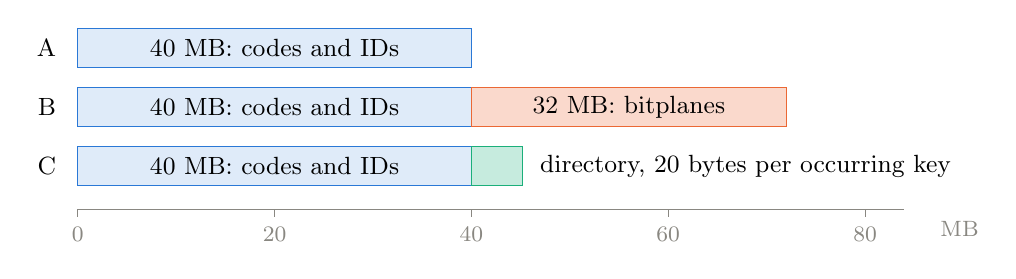
\begin{tikzpicture}
\foreach \y/\l in {1.5/A,0.75/B,0/C}{\node[anchor=east,font=\small] at (-.15,\y+.25) {\l};}
\draw[fill=Scan!15,draw=Scan](0,1.5)rectangle(5,2);\node[font=\small] at(2.5,1.75){40 MB: codes and IDs};
\draw[fill=Scan!15,draw=Scan](0,.75)rectangle(5,1.25);\node[font=\small] at(2.5,1){40 MB: codes and IDs};
\draw[fill=Branch!25,draw=Branch](5,.75)rectangle(9,1.25);\node[font=\small] at(7,1){32 MB: bitplanes};
\draw[fill=Scan!15,draw=Scan](0,0)rectangle(5,.5);\node[font=\small] at(2.5,.25){40 MB: codes and IDs};
\draw[fill=Keys!25,draw=Keys](5,0)rectangle(5.65,.5);\node[font=\small,anchor=west] at(5.75,.25){directory, 20 bytes per occurring key};
\draw[Muted] (0,-.3)--(10.5,-.3);\foreach \x/\l in {0/0,2.5/20,5/40,7.5/60,10/80}{\draw[Muted](\x,-.3)--(\x,-.4);\node[font=\footnotesize,text=Muted,below] at (\x,-.4){\l};}
\node[font=\footnotesize,text=Muted] at (11.2,-.55){MB};
\end{tikzpicture}
\caption{Index memory for one million 256-bit codes. Cluster centres, the hash table
overhead of C, and the working memory of a query are additional. The bitplane bar is for one
cluster; many small clusters add a little padding.}
\label{fig:memory}
\end{figure}

\subsection{Recall estimation}
The reference answer for a query is the top $K$ when every document is scored. Recall is
the share of those $K$ IDs that a method returns:
\[
 R=\frac{\text{reference IDs returned}}{K}.
\]
Returning 99 of the 100 reference documents is a recall of 99\%. This measures agreement
with the exact binary score, not whether a passage is a good answer to the question.

\subsubsection{Original method}
Method A scores every document in the opened clusters, so it can miss a reference document
only if that document's cluster was not opened. Let $r_{\rm route}(C,P)$ be the share of
reference documents that lie in the $P$ opened clusters, averaged over queries. Then
\[
 R_A=r_{\rm route}(C,P).
\]
This is a property of the clustering and the data, and Section~3 measures it directly.

\subsubsection{Bitplanes}
Method B can lose a document in a second way: by never scoring the group that holds it.
Writing $r_B$ for the share of reference documents inside the opened clusters that method B
actually returns,
\[
 R_B=r_{\rm route}(C,P)\times r_B.
\]
Without a node budget, $r_B=1$: the ceiling rule drops a group only when its ceiling
$Q-2p$ is below the $K$th best score already found, and such a group cannot contain a
top-$K$ document. In terms of the gap $g$ of Table~\ref{tab:symbols}, a group is skipped
exactly when its penalty exceeds $g$. In the running example the second-best score is
$1.9$, so $g=(2.5-1.9)/2=0.3$, and the group $\{2\}$ with penalty $0.5$ is skipped.
With a node budget, $r_B$ falls below one, and by how much depends on where the reference
documents sit in the split tree. That has no closed form; Section~4 measures it.

\subsubsection{Backward Walk}
The same reasoning gives
\[
 R_C=r_{\rm route}(C,P)\times r_C.
\]
$r_C=1$ when the walk runs until the ceiling rule stops it, because a key is skipped only
when its penalty exceeds $g$. A limit on lookups or on scored documents makes $r_C<1$.

The gap $g$ is the quantity that decides whether the new methods can skip anything. If no
reachable group or key has a penalty above $g$, both methods score every document that
method A scores and add their own work on top. Section~3 measures $g$ on the dataset and
compares it with the query weights that a split or a key flip can accumulate.

\subsection{Summary}
Tables~\ref{tab:time}, \ref{tab:memory} and \ref{tab:recall} collect the formulas. The
routing cost $T_{\rm route}$ and the constants $c_{\cdot}$ are measured in Section~4.

\begin{table}[H]\centering\small
\caption{Time for one query. $F$ counts scored documents; $V_s,V_l$ count 64-bit words
read while splitting and while collecting a group's documents; $G$ counts groups taken from
the queue; $H$ counts directory lookups and $E$ the keys visited.}
\label{tab:time}
\begin{tabularx}{\linewidth}{@{}lY@{}}\toprule
Method & Time formula\\\midrule
A: original & $T_A=T_{\rm route}+c_{\rm call}+c_{\rm score}F_A$, with $F_A=\sum_{\rm opened}n_c\approx NP/C$\\[3pt]
B: bitplanes & $T_B=T_{\rm route}+c_{\rm call}+c_{\rm score}F_B+c_{\rm split}V_s+c_{\rm leaf}V_l+c_{\rm group}G$, with $V_s=\sum_cJ_cW_c$, $V_l=\sum_cE_cW_c$\\[3pt]
C: backward walk & $T_C=T_{\rm route}+c_{\rm call}+c_{\rm score}F_C+c_{\rm lookup}H+c_{\rm key}E$, with $H=EP$ and $E\le2^h$\\\bottomrule
\end{tabularx}
\end{table}

\begin{table}[H]\centering\small
\caption{Index memory, for $d=256$. $U$ is the number of keys that occur in the data.}
\label{tab:memory}
\begin{tabularx}{\linewidth}{@{}lYY@{}}\toprule
Method & Index memory & Working memory per query\\\midrule
A: original & $M_A=40N$ bytes, plus $4Cd$ for cluster centres & lookup table and heap of $K$\\
B: bitplanes & $M_A+8d\sum_cW_c$ & table, heap, and one $8W_c$-byte mask per queued group\\
C: backward walk & $M_A+20U$, plus hash-table overhead & table, heap, and the queue of pending keys\\\bottomrule
\end{tabularx}
\end{table}

\begin{table}[H]\centering\small
\caption{Recall. $r_{\rm route}$ is the share of reference documents inside the opened
clusters; $r_B$ and $r_C$ are the shares of those that the local search returns.}
\label{tab:recall}
\begin{tabularx}{\linewidth}{@{}lYY@{}}\toprule
Method & Recall & When the local search loses nothing ($r=1$)\\\midrule
A: original & $r_{\rm route}(C,P)$ & always: every opened document is scored\\
B: bitplanes & $r_{\rm route}(C,P)\,r_B$ & no node budget; groups are dropped only when penalty $>g$\\
C: backward walk & $r_{\rm route}(C,P)\,r_C$ & no lookup or candidate limit; keys are dropped only when penalty $>g$\\\bottomrule
\end{tabularx}
\end{table}

\section{Deriving optima}
\newcommand{\gapShare}{15\xspace}
\newcommand{\gapShareMin}{9\xspace}
\newcommand{\gapShareMax}{21\xspace}
\newcommand{\gapOneShare}{9\xspace}
\newcommand{\topOneShare}{2.3\xspace}
\newcommand{\topTwelveShare}{15\xspace}
\newcommand{\topTwentyFourShare}{25\xspace}
\newcommand{\topSixtyFourShare}{52\xspace}
\newcommand{\splitsBeforePruning}{13\xspace}
\newcommand{\agreeRankOne}{99.9\xspace}
\newcommand{\agreeRankTwo}{86\xspace}
\newcommand{\agreeRankTwelve}{78\xspace}
\newcommand{\removedTwelve}{22\xspace}
\newcommand{\neighbourAgreeTwelve}{97\xspace}
\newcommand{\groupTwelveDocs}{124,689\xspace}
\newcommand{\groupTwelveShare}{12.5\xspace}
\newcommand{\groupTwelveNeighbours}{85\xspace}
\newcommand{\groupTwentyFourDocs}{9,305\xspace}
\newcommand{\groupTwentyFourNeighbours}{54\xspace}
\newcommand{\insideDocs}{325,353\xspace}
\newcommand{\insideAfterTwelve}{62,060\xspace}
\newcommand{\insideShareAfterTwelve}{19\xspace}
\newcommand{\insideNeighboursAfterTwelve}{84\xspace}
\newcommand{\keyFirstTwelveShare}{6.8\xspace}
\newcommand{\keyFirstTwelveDocs}{3,217\xspace}
\newcommand{\keyFirstTwelveNeighbours}{5\xspace}
\newcommand{\keyHeavyTwelveShare}{9.5\xspace}
\newcommand{\keyHeavyTwelveDocs}{302,372\xspace}
\newcommand{\keyHeavyTwelveNeighbours}{40\xspace}
\newcommand{\keyFirstEightShare}{5.2\xspace}
\newcommand{\probesEightyCfour}{72\xspace}
\newcommand{\docsEightyCfour}{18,107\xspace}
\newcommand{\docsShareEightyCfour}{1.8\xspace}
\newcommand{\probesNinetyCfour}{211\xspace}
\newcommand{\docsNinetyCfour}{52,164\xspace}
\newcommand{\docsShareNinetyCfour}{5.2\xspace}
\newcommand{\probesNinetyFiveCfour}{467\xspace}
\newcommand{\docsNinetyFiveCfour}{114,477\xspace}
\newcommand{\docsShareNinetyFiveCfour}{11.4\xspace}
\newcommand{\probesNinetyNineCfour}{1,330\xspace}
\newcommand{\docsNinetyNineCfour}{325,353\xspace}
\newcommand{\docsShareNinetyNineCfour}{32.5\xspace}
\newcommand{\probesEightyCeight}{127\xspace}
\newcommand{\docsEightyCeight}{15,615\xspace}
\newcommand{\docsShareEightyCeight}{1.6\xspace}
\newcommand{\probesNinetyCeight}{353\xspace}
\newcommand{\docsNinetyCeight}{42,847\xspace}
\newcommand{\docsShareNinetyCeight}{4.3\xspace}
\newcommand{\probesNinetyFiveCeight}{778\xspace}
\newcommand{\docsNinetyFiveCeight}{93,930\xspace}
\newcommand{\docsShareNinetyFiveCeight}{9.4\xspace}
\newcommand{\probesNinetyNineCeight}{2,440\xspace}
\newcommand{\docsNinetyNineCeight}{295,858\xspace}
\newcommand{\docsShareNinetyNineCeight}{29.6\xspace}

We now choose each method's settings for the dataset of Section~4: one million MS~MARCO
passages embedded with Nomic~v1.5, cut to 256 values and stored as 256 bits, with 200
queries and $K=100$. The requirement is the same for all three methods: return at least a
target share of the true top 100 (we use 80\%, 90\%, 95\% and 99\%), keep the index within
32~GB of RAM, and be as fast as possible. Memory turns out not to constrain anything here:
the largest index in Section~2 is under 100~MB. The choice is therefore made on time, and
each method may pick its own cluster count $C$, opened clusters $P$ and local settings. We
treat the methods one at a time and combine the results in Section~3.4.

\subsection{Original method}
Method A has two settings, $C$ and $P$, and one formula,
$T_A=T_{\rm route}(C,P)+c_{\rm call}+c_{\rm score}F_A(C,P)$. The recall requirement
removes one degree of freedom: for each $C$, $P$ must be the smallest number of clusters
that contains the target share of the reference documents. That number comes from the data.
We rank every cluster by its distance to each query, note the rank of the cluster that holds
each reference document, and read off how many clusters must be opened to reach each
target. Figure~\ref{fig:routing} shows the result as recall against documents opened, and
Table~\ref{tab:routing} lists the values at the four targets.

\begin{figure}[htb]\centering
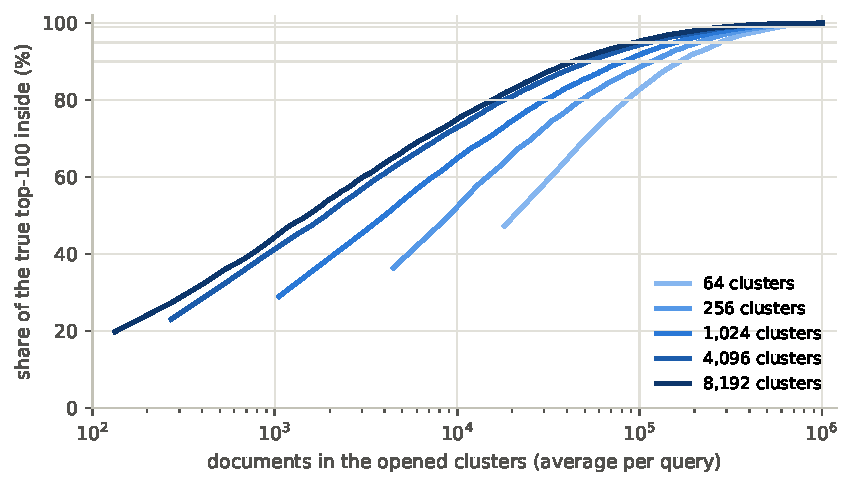
\includegraphics[width=.74\linewidth]{figures/routing.pdf}
\caption{Share of the true top-100 that lies in the opened clusters, against the number of
documents those clusters contain, for five cluster counts on the dataset. Horizontal lines
mark the four recall targets. More clusters reach a target with fewer documents, because the
opened region fits the query more tightly.}
\label{fig:routing}
\end{figure}

\begin{table}[htb]\centering\small
\caption{Clusters $P$ that must be opened, and documents those clusters hold on average,
for each recall target and cluster count. These are the $F_A$ values of the time formula.}
\label{tab:routing}
\begin{tabular}{@{}rrrrrrrrr@{}}\toprule
Clusters $C$ & \multicolumn{2}{c}{80\%} & \multicolumn{2}{c}{90\%} & \multicolumn{2}{c}{95\%} & \multicolumn{2}{c}{99\%}\\
 & $P$ & docs & $P$ & docs & $P$ & docs & $P$ & docs\\\midrule
64 & 6 & 98,610 & 11 & 178,239 & 18 & 286,892 & 37 & 580,487\\
256 & 12 & 50,005 & 29 & 118,453 & 52 & 211,419 & 119 & 480,127\\
1,024 & 31 & 30,626 & 84 & 82,157 & 164 & 160,584 & 420 & 412,040\\
4,096 & 72 & 18,107 & 211 & 52,164 & 467 & 114,477 & 1,330 & 325,353\\
8,192 & 127 & 15,615 & 353 & 42,847 & 778 & 93,930 & 2,440 & 295,858\\
\bottomrule\end{tabular}

\end{table}

Two effects pull in opposite directions as $C$ grows. The scoring term
$c_{\rm score}F_A$ falls, because Table~\ref{tab:routing} shows fewer documents for the
same recall: at 99\%, 574,000 documents with 64 clusters against 296,000 with 8,192.
The routing term rises, because selecting clusters compares the query with all $C$ centres,
$256C$ multiplications, and then sorts out the best $P$. Writing $T_{\rm route}\approx
c_{\rm centre}C+c_{\rm sort}P\log P$, the time is smallest where
\[
 \frac{dT_A}{dC}=c_{\rm centre}+c_{\rm score}\frac{dF_A}{dC}=0,
\]
that is, where opening one more cluster's worth of routing costs as much as the scoring it
saves. The recall curve flattens at high targets (the last few reference documents are
spread over many clusters), so $F_A$ stops falling quickly beyond a few thousand clusters,
while $c_{\rm centre}C$ keeps growing. With $c_{\rm score}\approx27$~ns per document
(Section~4) and a centre comparison of the same order, the formula puts the optimum at
$C=4{,}096$ or $8{,}192$ for every target: the difference in $F_A$ between them is worth
about 0.7~ms at 99\% and only 0.07~ms at 80\%, against roughly 0.1~ms of extra routing.
Section~4 measures both.

\subsection{Bitplanes}
Method B starts from the same clusters and adds two settings, the leaf size $L$ and the
node budget. At the same $C$ and $P$ the two time formulas differ by
\begin{equation}
 T_B-T_A=c_{\rm split}V_s+c_{\rm leaf}V_l+c_{\rm group}G-c_{\rm score}(F_A-F_B).
 \label{eq:bdiff}
\end{equation}
Method B wins only if the last term, the scoring it avoids, is larger than the three mask
terms. Two questions decide the size of $F_A-F_B$: how many documents does one split remove,
and may the removed group be skipped at all?

\textbf{How much a split removes.} A split keeps the documents whose bit agrees with the
query sign at one position. If document signs were balanced, half of a group would go each
way and twelve splits would cut a million documents to about 244. On this dataset the signs
are not balanced. Figure~\ref{fig:split} shows the share of documents removed by keeping the
preferred sign at each position, ordered by the query's weight. At the position with the
largest weight only \agreeRankOne\% of documents agree with the query and \(0.1\%\) are
removed; this position carries the same sign in almost every document and query, so it says
nothing about which documents are close. At the next eleven positions a split removes
between 14\% and \removedTwelve\%. After the twelve largest weights, \groupTwelveShare\% of
the collection is still in the group, \groupTwelveDocs\ documents instead of 244. Inside
the clusters opened for 99\% recall the effect is weaker still: those documents already
resemble the query, and twelve splits keep \insideShareAfterTwelve\% of them.

\begin{figure}[htb]\centering
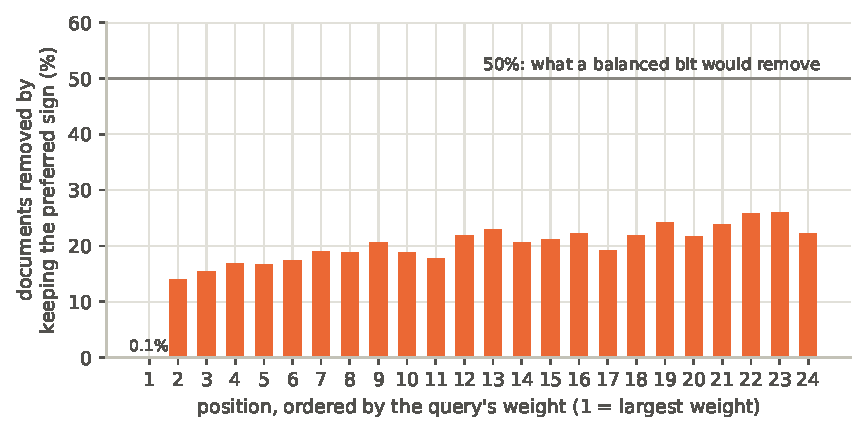
\includegraphics[width=.74\linewidth]{figures/split-removes.pdf}
\caption{What one split removes on this dataset, by the rank of the query weight at the
split position, averaged over the 200 queries. A balanced bit would remove 50\%. Real
embeddings agree with the query on its heavy positions far more often than not, so each
split removes a small minority.}
\label{fig:split}
\end{figure}

\textbf{Whether the removed group may be skipped.} Without a budget, method B drops a group
only when its penalty exceeds the gap $g$ (Section~2.3). On this dataset the gap averages
\gapShare\% of the total weight $Q$ (between \gapShareMin\% and \gapShareMax\% across
queries), while the largest single weight is only \topOneShare\% of $Q$ and the twelve
largest together are \topTwelveShare\%. A group that disagrees with the query at one heavy
position therefore has a penalty far below $g$, and the search must visit it. Adding up the
weights in order, a group would need to disagree at about \splitsBeforePruning\ of the
heaviest positions before the ceiling rule could drop it, and by then it holds almost
nothing. In the exact mode, then, $F_B=F_A$: every document that method A scores, method B
scores too, after paying for the masks. Equation~\ref{eq:bdiff} is minimised by making no
splits at all, $L\ge n_c$, which leaves
\[
 T_B-T_A=c_{\rm leaf}\sum_{c\ \text{opened}}W_c+c_{\rm group}P>0.
\]

\textbf{With a budget.} A node budget stops the search early and turns method B into an
approximate filter: it scores the groups that agree with the most heavy signs and drops the
rest, losing the reference documents in them. Whether that is a good trade depends on how
well ``agrees with the heavy signs'' predicts ``is a true neighbour'', compared with the
filter method A already has, ``is in a nearby cluster''. Figure~\ref{fig:filters} plots both
on the same axes: documents kept against true neighbours kept. Twelve splits keep
\groupTwelveShare\% of the documents and \groupTwelveNeighbours\ of the 100 neighbours;
opening the \probesEightyCfour closest of 4,096 clusters keeps \docsShareEightyCfour\%
of the documents and 80 neighbours. Clusters are the sharper filter at every point, so any
recall that a budget gives up is recovered more cheaply by opening fewer clusters. Method B
with a budget cannot beat method A here either.

\begin{figure}[htb]\centering
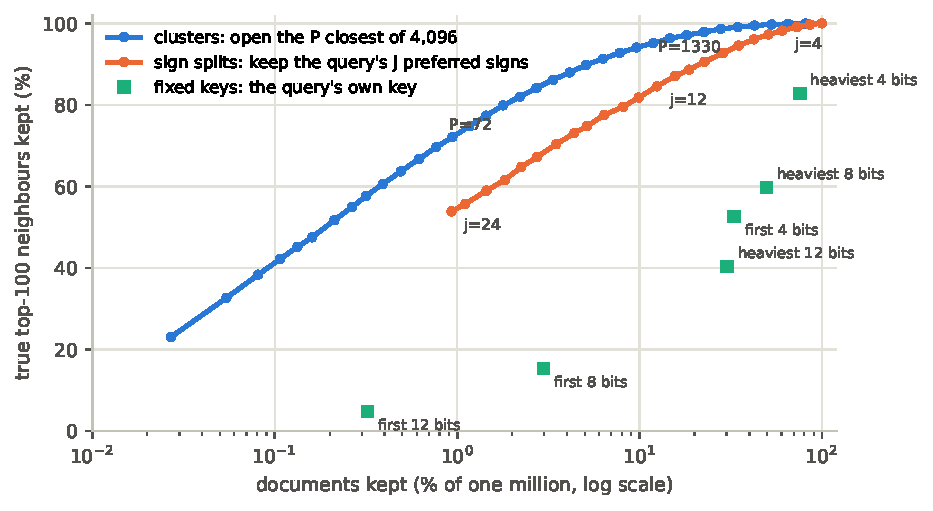
\includegraphics[width=.74\linewidth]{figures/filter-quality.pdf}
\caption{Three ways to keep only part of the collection, on the same dataset. A good filter
sits high and to the left: few documents kept, many true neighbours kept. Cluster selection
(blue) dominates sign splits (orange) and fixed keys (green) at every level.}
\label{fig:filters}
\end{figure}

\textbf{When Bitplanes would win.} The formula also says what a dataset must look like for
the mask work to pay. Two conditions are needed together: a split at a heavy position must
remove a large share of the group (balanced signs), and the heaviest few weights must
exceed the gap, $\sum_{i\le j}|q_{(i)}|>g$ for a small $j$, so that the ceiling drops the
other child. When both hold, one path of $j$ splits reads $jW$ words and scores about
$n2^{-j}$ documents; with $c_{\rm split}$ near half a nanosecond per word and
$c_{\rm score}$ near 27~ns per document, that path is cheaper than scoring the cluster as
soon as $j$ is a few units, by a factor that grows like $2^{j}$. Queries whose weight is
concentrated in a dozen positions that change from query to query are the case in which
method B is designed to shine. This dataset's queries spread their weight over hundreds of
positions.

\subsection{Backward Walk}
Method C adds the key width $h$. At the same clusters,
\begin{equation}
 T_C-T_A=c_{\rm lookup}H+c_{\rm key}E-c_{\rm score}(F_A-F_C),
\end{equation}
and the walk skips a key only when its penalty exceeds the gap $g$. The largest penalty a
key can have is the total weight of the $h$ key positions, so the question is whether those
fixed positions carry more than \gapShare\% of $Q$. They do not. The first eight positions
carry \keyFirstEightShare\% of the query weight on average and the first twelve
\keyFirstTwelveShare\%; even the twelve positions with the largest average weight across
all queries carry only \keyHeavyTwelveShare\%. No key is ever skipped, so the walk visits all
$2^h$ keys, $H=2^hP$, and $F_C=F_A$. The difference is minimised by the narrowest key:
$h=4$ costs $16P$ lookups on top of method A. Any wider key adds lookups without removing
scoring.

A limit on scored documents would make method C an approximate filter, like a budget for
method B. Figure~\ref{fig:filters} shows how the query's own key performs in that role.
With the first twelve positions as the key, the query's key holds \keyFirstTwelveDocs\
documents but only \keyFirstTwelveNeighbours\ of the 100 true neighbours: a key built from
light positions selects documents that agree where it hardly matters. With the twelve
heaviest positions, the key holds \keyHeavyTwelveDocs\ documents and
\keyHeavyTwelveNeighbours\ neighbours, because those positions are the ones almost every
document shares. Either way the key is a far worse filter than the clusters, so a candidate
limit cannot make method C competitive on this dataset.

\textbf{When Backward Walk would win.} Method C needs what method B needs, with one more
condition: the heavy positions must be the same for every query, because the key positions
are fixed when the index is built. Given that, a directory lookup is cheaper than a mask
split, and method C would reach the small group in one lookup where method B needs $h$
splits.

\subsection{Comparison}
Table~\ref{tab:conditions} collects the conditions and the dataset's values.
Both new methods can only remove scoring work when a small set of query positions is heavy
enough to exceed the gap and balanced enough to split the documents. On this dataset
neither condition holds, so the formulas predict, for every recall target, the order
\[
 T_A<T_B\ (\text{no splits})<T_C\ (h=4),
\]
with method B and C behind by their bookkeeping only: about $c_{\rm leaf}\sum W_c+
c_{\rm group}P$ for B and $16\,c_{\rm lookup}P$ for C. At the 99\% target with $C=4{,}096$
and $P=\probesNinetyNineCfour$, those are fractions of a millisecond on top of about
$c_{\rm score}\times\docsNinetyNineCfour\approx9$~ms of scoring. Table~\ref{tab:regions}
states where each method is expected to be fastest in general. Section~4 tests the
prediction for this dataset.

\begin{table}[htb]\centering\small
\caption{What each new method needs in order to skip scoring work, and what this dataset
provides. $g$ is the gap of Table~\ref{tab:symbols}, averaged over queries.}
\label{tab:conditions}
\begin{tabularx}{\linewidth}{@{}YlYc@{}}\toprule
Condition & Needed by & This dataset & Met\\\midrule
Heaviest few weights exceed the gap: $\sum_{i\le j}|q_{(i)}|>g$ for small $j$ & B and C & 12 heaviest weights: \topTwelveShare\% of $Q$; gap: \gapShare\% of $Q$; \splitsBeforePruning\ positions needed & no\\
A split on a heavy position removes about half the group & B and C & removes 0.1\% at the heaviest position, 14--\removedTwelve\% at the next eleven & no\\
The heavy positions are the same for every query & C only & first 12 positions: \keyFirstTwelveShare\% of $Q$; 12 heaviest on average: \keyHeavyTwelveShare\% & no\\
A cluster boundary is a weak filter, so local pruning has work left to save & B and C & \probesEightyCfour of 4,096 clusters hold 80 of 100 neighbours in \docsShareEightyCfour\% of the documents & no\\\bottomrule
\end{tabularx}
\end{table}

\begin{table}[htb]\centering\small
\caption{Where each method is expected to be fastest, from the formulas of Section~2.}
\label{tab:regions}
\begin{tabularx}{\linewidth}{@{}lY@{}}\toprule
Fastest & Situation\\\midrule
A: original & Query weight is spread over many positions, or documents mostly share the query's sign at its heavy positions. No group or key can be dropped, so extra structure only adds work. This dataset.\\
B: bitplanes & A few heavy positions carry more weight than the gap, their signs split the documents evenly, and which positions are heavy changes from query to query. Splits follow each query's own order.\\
C: backward walk & The same as B, but the heavy positions are the same for all queries, so a fixed key captures them and one lookup replaces several splits.\\\bottomrule
\end{tabularx}
\end{table}

\section{Experiments}
\newcommand{\msEightyScan}{0.57}
\newcommand{\msEightyBranch}{0.58}
\newcommand{\msEightyKeys}{0.62}
\newcommand{\msNinetyScan}{1.44}
\newcommand{\msNinetyBranch}{1.50}
\newcommand{\msNinetyKeys}{1.74}
\newcommand{\msNinetyFiveScan}{2.87}
\newcommand{\msNinetyFiveBranch}{3.02}
\newcommand{\msNinetyFiveKeys}{3.69}
\newcommand{\msNinetyNineScan}{8.70}
\newcommand{\msNinetyNineBranch}{9.02}
\newcommand{\msNinetyNineKeys}{11.13}
\newcommand{\ratioBoverA}{1.04}
\newcommand{\ratioCoverA}{1.28}
\newcommand{\unitErrorScan}{1.7}
\newcommand{\unitWorstScan}{8}
\newcommand{\unitErrorBranch}{13.7}
\newcommand{\unitWorstBranch}{75}
\newcommand{\unitErrorKeys}{8.0}
\newcommand{\unitWorstKeys}{38}
\newcommand{\scoreMicroseconds}{0.026}
\newcommand{\splitNanoseconds}{0.3}
\newcommand{\lookupNanoseconds}{13}
\newcommand{\settingsMeasured}{189}
\newcommand{\globalScanMs}{26.8}
\newcommand{\globalBranchMs}{745}
\newcommand{\globalBranchSplitWords}{291}
\newcommand{\globalBranchGroups}{36,983}

The experiment has two jobs: check that the code does the work the formulas count, and find
which method is fastest at each recall target. Everything is measured on one machine, an
Apple M5~Max with 128~GiB of RAM, using one CPU thread and one query at a time.

\subsection{Setup}
The inputs are fixed and identical for every setting. The documents are one million
MS~MARCO passages~\cite{msmarco}, embedded with Nomic Embed v1.5~\cite{nomic}, cut to the
first 256 values and stored as 256 sign bits. The 200 queries come from the same collection's
development set. The reference answer for each query is its exact top 100 when all one
million documents are scored. The arrays are read in place; their hashes are recorded before
and after the run and did not change.

What varies is only the index. We use the cluster counts $C\in\{64,256,1024,4096,8192\}$,
with cluster centres learned once by $k$-means~\cite{faiss}, plus the whole collection as a
single cluster. For each $C$, $P$ takes the four values from Table~\ref{tab:routing}, one
per recall target. Every method is measured on all 21 resulting $(C,P)$ pairs, so no
method gets a routing advantage. Within each pair, method A has no further settings; method B
is run without splits, with leaf size 128 and no budget, and with leaf size 128 and node
budgets of 64, 512 and 4,096; method C is run with key widths 4, 8 and 12. That gives
\settingsMeasured\ settings. Each runs in its own process, builds its index from the same
codes, answers the 200 queries twice (once for the slowest setting), and records for every
query the time, the returned IDs and the operation counts of Section~2. We report the median
time over the 400 timings and the mean recall over the 200 queries. The largest process
peak was 1.5~GB, far below the 32~GB limit, so every setting is eligible.

\subsection{Checking the calculations}
Table~\ref{tab:checks} compares the counts that Section~2 predicts from the data and the
settings with the counts the code recorded. Every one matches: the documents scored equal
the documents in the opened clusters, the recall of an exact setting equals the routing
recall $r_{\rm route}$, method B without splits reads exactly $\sum_cW_c$ leaf words, method
C visits all $2^h$ keys and makes $2^hP$ lookups, and the index sizes are the byte counts of
Section~2.2. The work formulas are therefore a correct description of the code.

\begin{table}[htb]\centering\small
\caption{Predicted against recorded counts over the \settingsMeasured\ settings. ``None''
means every setting agreed exactly.}
\label{tab:checks}
\begin{tabular}{@{}lrr@{}}\toprule
Quantity (formula) & Settings checked & Largest difference\\\midrule
Documents scored, $F$ (exact settings) & 126 & 0.00\%\\
Recall $=r_{\rm route}$ (exact settings) & 126 & none\\
Leaf words $V_l$ (B without splits) & 21 & none\\
Split words $V_s$ (B without splits) & 21 & none\\
Keys visited $E=2^h$ & 63 & none\\
Lookups $H=2^hP$ & 63 & none\\
Code bytes $=32N$ & 189 & none\\
ID bytes $=8N$ & 189 & none\\
Bitplane bytes $=8d\sum_cW_c$ & 105 & none\\
Directory bytes $=20U$ & 63 & none\\
\bottomrule\end{tabular}

\end{table}

Turning counts into time needs the constants $c_{\cdot}$. We fit them by least squares on
the measured search times of each method's settings, weighting each setting by its own time
so that fast and slow settings count equally (Table~\ref{tab:units}). Scoring one document
costs about \scoreMicroseconds~$\mu$s in all three methods, a directory lookup about
\lookupNanoseconds~ns, a split word well under a nanosecond, and taking a group from the
queue about a quarter of a microsecond. Figure~\ref{fig:predicted} plots the time the
formula gives against the time measured. For method A the median error is
\unitErrorScan\%, for method C \unitErrorKeys\%, and for method B without splits 11\%.

\begin{table}[htb]\centering\small
\caption{Unit costs from the fit, in microseconds, and the median absolute error of the
fitted formula over each method's settings.}
\label{tab:units}
\begin{tabular}{@{}llrrr@{}}\toprule
Method & Cost & Microseconds & Settings & Median error\\\midrule
A: original & per call, $c_{\rm call}$ & 45.8228 & 21 & 1.7\%\\
 & per scored document, $c_{\rm score}$ & 0.0260 & & \\
B: bitplanes & per call, $c_{\rm call}$ & 9.2597 & 105 & 13.7\%\\
 & per scored document, $c_{\rm score}$ & 0.0295 & & \\
 & per split word, $c_{\rm split}$ & 0.0003 & & \\
 & per leaf word, $c_{\rm leaf}$ & 0.0032 & & \\
 & per group taken from the queue, $c_{\rm group}$ & 0.2394 & & \\
C: backward walk & per call, $c_{\rm call}$ & 11.0438 & 63 & 8.0\%\\
 & per scored document, $c_{\rm score}$ & 0.0308 & & \\
 & per directory lookup, $c_{\rm lookup}$ & 0.0132 & & \\
 & per key generated, $c_{\rm key}$ & 0.0000 & & \\
\bottomrule\end{tabular}

\end{table}

\begin{figure}[htb]\centering
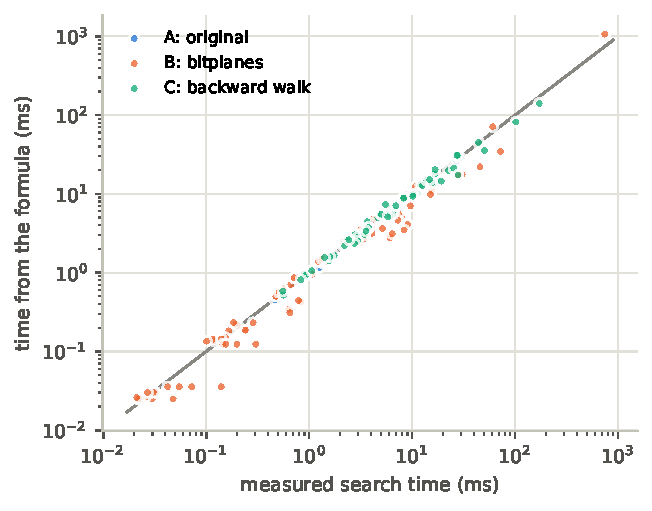
\includegraphics[width=.5\linewidth]{figures/predicted-vs-measured.pdf}
\caption{Search time computed from the recorded counts and the unit costs of
Table~\ref{tab:units}, against the measured median. Points on the grey line are exact.}
\label{fig:predicted}
\end{figure}

The formula is least accurate for method B when it splits wide clusters. At $C=64$ with 37
opened clusters and leaf size 128 the measured time is 72~ms against 35~ms from the formula,
and the single-cluster search with leaf size 128 takes \globalBranchMs~ms against
\globalBranchSplitWords\ million split words and \globalBranchGroups\ groups. The counts
are right; the constants are not constant. When many groups wait in the queue, their masks
and the bitplanes no longer fit in the processor caches, and each word costs several times
more than in the small-cluster settings that dominate the fit. The error runs in one
direction only: splitting is more expensive than the formula says, so it does not change the
comparison below.

\subsection{Results}
Table~\ref{tab:selected} and Figure~\ref{fig:results} give, for each recall target, the
fastest setting of each method that reached the target. Method A is fastest at all four
targets. Method B is behind by 1\% to 4\%, and its fastest setting at every target is the one
without splits, as Section~3.2 derived. Method C is behind by 9\% to 28\% with its narrowest
key, $h=4$, as Section~3.3 derived. All three methods score the same documents at the same
$(C,P)$; the differences are the bookkeeping that Section~3.4 predicted, about
$0.4$~$\mu$s per opened cluster for B and $16$ lookups per opened cluster for C.

\begin{table}[htb]\centering\small
\caption{Fastest setting of each method at each recall target, over all measured settings
that reached the target. Recall is the mean over 200 queries; time is the median per query
including cluster selection.}
\label{tab:selected}
\begin{tabularx}{\linewidth}{@{}llYrrr@{}}\toprule
Target & Method & Setting & Recall & Median ms & Docs scored\\\midrule
80\% & A: original & $C=4,096$, $P=72$ & 80.01\% & 0.569 & 18,107\\
 & B: bitplanes & $C=4,096$, $P=72$; no splits & 80.01\% & 0.576 & 18,107\\
 & C: backward walk & $C=4,096$, $P=72$; $h=4$ & 80.01\% & 0.621 & 18,107\\
\addlinespace[2pt]
90\% & A: original & $C=8,192$, $P=353$ & 90.02\% & 1.442 & 42,847\\
 & B: bitplanes & $C=8,192$, $P=353$; no splits & 90.02\% & 1.496 & 42,847\\
 & C: backward walk & $C=8,192$, $P=353$; $h=4$ & 90.02\% & 1.741 & 42,847\\
\addlinespace[2pt]
95\% & A: original & $C=8,192$, $P=778$ & 95.00\% & 2.872 & 93,930\\
 & B: bitplanes & $C=8,192$, $P=778$; no splits & 95.00\% & 3.022 & 93,930\\
 & C: backward walk & $C=8,192$, $P=778$; $h=4$ & 95.00\% & 3.693 & 93,930\\
\addlinespace[2pt]
99\% & A: original & $C=4,096$, $P=1,330$ & 99.00\% & 8.702 & 325,353\\
 & B: bitplanes & $C=8,192$, $P=2,440$; no splits & 99.00\% & 9.023 & 295,858\\
 & C: backward walk & $C=8,192$, $P=2,440$; $h=4$ & 99.00\% & 11.130 & 295,858\\
\addlinespace[2pt]
\bottomrule\end{tabularx}

\end{table}

\begin{figure}[htb]\centering
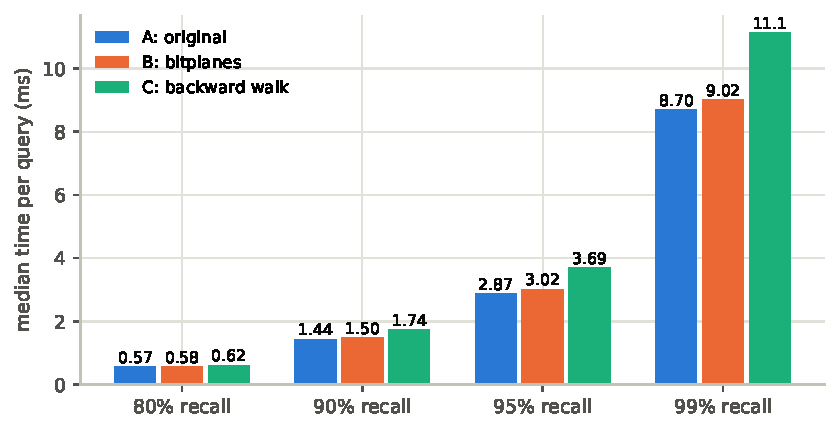
\includegraphics[width=.7\linewidth]{figures/results.pdf}
\caption{The same fastest settings as Table~\ref{tab:selected}. Lower is better.}
\label{fig:results}
\end{figure}

The other settings show the rest of the prediction. For method A, $C=4{,}096$ and
$8{,}192$ are within 1\% of each other at 99\% (8.70 and 8.78~ms), while 64 clusters take
14.9~ms: fewer clusters open more documents, as Table~\ref{tab:routing} says. Cluster
selection itself costs 0.07~ms for 4,096 centres and 0.14~ms for 8,192, growing to 0.37~ms
when 2,440 of them must be sorted out, which is why 4,096 wins at 80\% and 99\% and 8,192
at 90\% and 95\%. For method B, splitting always costs more than it saves: with leaf size
128 and no budget the 99\% setting takes 11.1~ms instead of 9.0, and the 80\% setting
0.79~ms instead of 0.58, because $F_B=F_A$ and the masks are pure overhead. With a budget
the search is faster but loses most of the answer: at $C=8{,}192$, $P=2{,}440$ a budget of
4,096 groups reaches 44\% recall in 5.5~ms and a budget of 512 reaches 37\% in 1.4~ms,
while method A reaches 80\% in 0.57~ms by opening fewer clusters. The best budgeted
setting that reaches 80\% takes 0.72~ms, still behind A. For method C, every extra key bit
doubles the lookups: at the 99\% clusters $h=4$, 8 and 12 take 11.1, 28.3 and 172~ms.
Figure~\ref{fig:all} shows all \settingsMeasured\ settings together.

\begin{figure}[htb]\centering
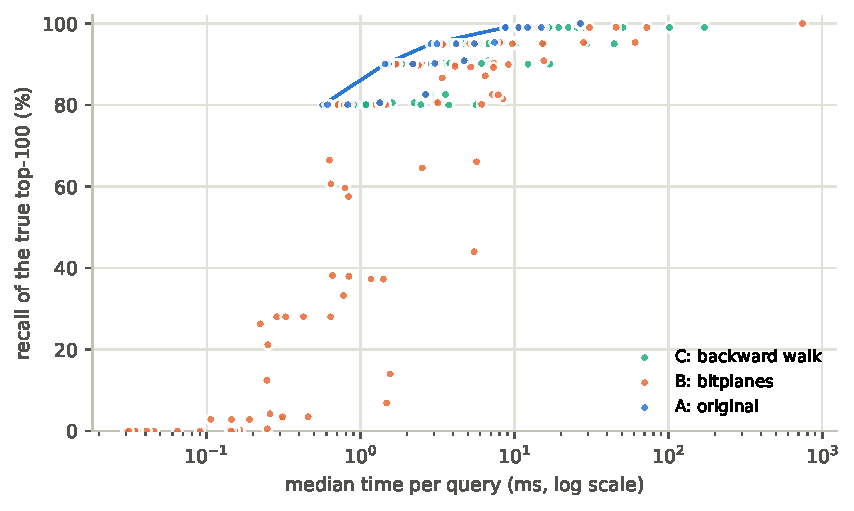
\includegraphics[width=.7\linewidth]{figures/all-settings.pdf}
\caption{Every measured setting. The blue line joins method A's fastest settings at the four
targets. Orange points below 80\% are budgeted bitplane searches; green points beyond 20~ms
are backward walks with wide keys.}
\label{fig:all}
\end{figure}

\subsection{Code references}
The search code is \path{cpp/index.cpp} (method A in \texttt{Index::scan}, method B in
\texttt{Index::search}), \path{cpp/key_index.cpp} (method C) and \path{cpp/score.hpp}
(the shared lookup-table scorer, top-$K$ heap and ceiling rule). The experiment is
\path{experiments/fixed_data_study.py}; each setting is measured by
\path{experiments/worker.py}. The run, with every per-query record, is under
\path{results/fixed-data-2026-09-12/}: \texttt{settings.csv} has one row per setting,
\texttt{selected.csv} the fastest per method and target, \texttt{checks.json} the count
comparisons and \texttt{unit-costs.json} the fit. To repeat the run on this machine:
\begin{lstlisting}
.venv/bin/python -m experiments.fixed_data_study run --output results/my-run
.venv/bin/python reports/search-fixed-data/make_results.py facts
.venv/bin/python reports/search-fixed-data/make_results.py results --run results/my-run
bash reports/search-fixed-data/build.sh
\end{lstlisting}

\section{Limitations and next steps}
The result holds for one dataset, one embedding model and one code width. The two
properties that decided it, how much weight a query puts on its heaviest positions and how
often documents share the query's sign there, are properties of the embedding model. A
model whose queries concentrate their weight in a few positions, or a code whose bits are
closer to balanced, would move the dataset in Table~\ref{tab:conditions} and could change
the winner. The natural next step is to measure those two properties for other embedding
models before building any index; both take minutes on a sample and Section~3 shows how to
read them.

The time formula for method B is exact in its counts but optimistic in its constants when
clusters are wide, because the per-word cost depends on cache behaviour. A model that
prices cold masks separately would fit better; it would make splitting look worse, not
better. The single-thread, single-query measurement also leaves out batching and
multi-core effects that a production system would have.

Some design choices were not explored. Method C used contiguous key positions; choosing the
positions with the largest average weight is possible but, on this dataset, still leaves
the key well below the gap. Method B could store sparse masks instead of full-width ones,
which would lower its constant but not create documents to skip. Finally, all results are
for $K=100$; a smaller $K$ makes the gap smaller and pruning slightly easier, but not by
enough to cross the threshold here.

\section{Conclusion}
We compared Exa's cluster-then-scan search with two additions that try to skip scoring
work, on one fixed dataset with only the index parameters varied. The calculations of
Section~2 describe the code exactly: every predicted operation count matched the recorded
one. The derivation of Section~3 predicted that neither addition can skip anything on this
dataset, because a single sign bit removes only 14\% to 22\% of the documents and no group
or key ever exceeds the gap that would let the ceiling rule drop it. The measurements of
Section~4 confirmed the prediction: the original method was fastest at every recall target,
Bitplanes was 1\% to 4\% slower with its best setting being ``no splits'', and Backward
Walk was 9\% to 28\% slower with its narrowest key.

The methods are not useless; they are aimed at a different kind of data. Bitplanes win
when a few heavy query positions exceed the gap and split the documents evenly, and Backward
Walk wins when, in addition, those positions are the same for every query. The formulas
give those conditions in a form that can be checked on a sample before an index is built,
which is the practical outcome of this study.

\begin{thebibliography}{9}\small\raggedright
\bibitem{exa} Exa Team. \emph{How we built a web-scale vector database}. 2024.
\url{https://exa.ai/blog/building-web-scale-vector-db}.
\bibitem{mrl} A.~Kusupati et al. \emph{Matryoshka Representation Learning}. NeurIPS 2022.
\url{https://arxiv.org/abs/2205.13147}.
\bibitem{nomic} Z.~Nussbaum, J.~X.~Morris, B.~Duderstadt and A.~Mulyar. \emph{Nomic Embed:
Training a Reproducible Long Context Text Embedder}. 2024.
\url{https://arxiv.org/abs/2402.01613}.
\bibitem{msmarco} P.~Bajaj et al. \emph{MS MARCO: A Human Generated MAchine Reading
COmprehension Dataset}. 2016. \url{https://arxiv.org/abs/1611.09268}.
\bibitem{faiss} M.~Douze et al. \emph{The Faiss library}. 2024.
\url{https://arxiv.org/abs/2401.08281}.
\end{thebibliography}

\end{document}
